% !TeX spellcheck = en_US

\chapter{Project Progress}

At the very beginning of this project a detailed project plan has been defined. We divided each feature into a list of subsequent tasks and estimated the work required to complete them. 

This chapter reviews the progress throughout the project. At the each release we analyze how much time has been spent on the single tasks and if our initial planning needs to be adapted.


\section{Alpha Release: 22.12.2016}

The goal was to implement feature 1 (Transmission Chain) and feature 2 (RDS Transmission). This goal has been achieved. Additionally we started to document the implementation, which was initially planned to be done at the end of the project. 

\begin{table}[!htbp]
\centering
\caption{Expected and Actual Workload for Features in Alpha Release}
\label{tab:alpha:features}
\begin{tabular}{ l | c | c }
	 & expected  & actual \\ \hline
	Transmission Chain & 50h & 24h \\  \hline
	RDS Transmission & 35h & 55h \\ \hline
	Documentation & 0h & 7h \\ \hline \hline
	Total & 85h & 86h 
\end{tabular}
\end{table}

Table~\ref{tab:alpha:features} shows the total workloads that were required to implement the features. We can see that we overestimated the transmission chain feature and underestimated the RDS feature. In total the required time is roughly as expected. 

\begin{table}[!htbp]
	\centering
	\caption{Expected and Actual Workload for Feature 1: Transmission Chain}
	\label{tab:alpha:feature1}
	\begin{tabular}{ l | c | c }
		& expected  & actual \\ \hline
		Task 1: Investigation of Existing Code & 5h & 3h \\  \hline
		Task 2: Rewrite Modulator  & 10h & 9h \\ \hline
		Task 3: Implementation Interpolator & 10h & 0h \\ \hline
		Task 4: Refactor Existing Code and Finalize & 5h& 2h  \\ \hline
		Task 5: Integration & 10h & 4h  \\ \hline
		Task 6: Regression Testing & 10h & 6h  \\ \hline \hline 
		Total & 50h & 24h 
	\end{tabular}
\end{table}

Table~\ref{tab:alpha:feature1} lists the single tasks for feature 1. We decided to leave out the interpolator at first (see Section~\ref{sec:impl:feature1}). All other tasks were much easier as expected. Even the integration and testing with the already existing transmission modes went very well. 
	
	\begin{table}[!htbp]
		\centering
		\caption{Expected and Actual Workload for Feature 2: RDS Transmission}				\label{tab:alpha:feature2}
		\begin{tabular}{ l | c | c }
			& expected  & actual \\ \hline
			Task 7: Investigation of Existing Code&  5h & 5h \\ \hline
			Task 8: Implementation in MATLAB & 5h & 6h  \\ \hline
			Task 9: Portation to Java & 15h & 17h  \\ \hline
			Task 10: Testing and Bug Fixing & 10h & 26h \\ \hline \hline
			Total & 35h & 55h
		\end{tabular}
	\end{table}
	
	Table~\ref{tab:alpha:feature2} evaluates the required time for the tasks in feature 2. Tasks 7, 8 and 9 were nearly completed within the expected time, while the testing and debugging took much longer than expected. We highly underestimated the complexity of finding bugs in signal processing code on Android. Since we are dependent on the HackRF hardware and driver, most of the testing needs to be done on the actual smartphone. This means that it requires a lot of manual work - although we tried to implement some automated testing (see \ref{sec:impl:feature2}). 
	
	\begin{figure}[!htbp]
		\centering
		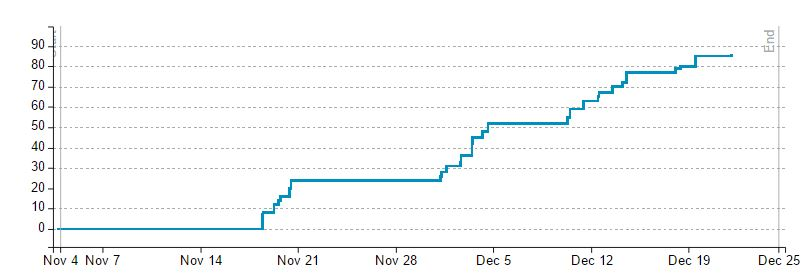
\includegraphics[width=1\linewidth]{gfx/Agilefant_Alpha.jpg}
		\caption{Workload Distribution for Alpha Release (04.11.2016-22.12.2016)}
		\label{fig:agilefant_alpha}
	\end{figure}
	
	Figure~\ref{fig:agilefant_alpha} gives the distribution of the workload as exported from our tracking tool Agilefant. The workload was not well distributed at the beginning, mainly focused on single weekends with long breaks in between. During the last weeks before the deadline this became slightly more distributed. 

\section{Beta Release: 02.02.2017}
The (ambitious) goal of this release was to finish all remaining features. This goal was not achieved, due to lack of time. However, we already finished a good portion of the documentation, which was initially planned for the final release. 

\begin{table}[!htbp]
	\centering
	\caption{Expected and Actual Workload for Features in Beta Release}
	\label{tab:beta:features}
	\begin{tabular}{ l | c | c }
		& expected  & actual \\ \hline
		Walkie Talkie & 60h & 65h \\  \hline
		BPSK Demodulation Improvement & 55h & 0h \\  \hline
		Documentation & 0h & 13h \\ \hline \hline
		Bug Fixing of previous features & 0h & 10h \\ \hline \hline 
		Total & 115h & 88h 
	\end{tabular}
\end{table}
Table~\ref{tab:beta:features} shows the expected and actual time spent implementing the features. The Walkie Talkie was expected to take 60 hours and was completed in 65 hours. The BPSK feature was expected to take 55 hours, but it was decided to exclude this feature, because the benefit of an improved BPSK demodulation implementation is not high enough. 
Additionally, we spent 13 hours creating this documentation and needed 10 unplanned hours to fix problems in the transmission chain and RDS implementation. In total we have spent 88 hours which is way below the planned value of 115 hours. 



	\begin{table}[!htbp]
	\centering
	\caption{Expected and Actual Workload for Feature 4: Walkie Talkie}
	\label{tab:alpha:feature4}
	\begin{tabular}{ l | c | c }
		& expected  & actual \\ \hline
		Task 17: Design and Implement UI& 15h & 19h \\ \hline
		Task 18: Implementation AM& 15h & 0h  \\ \hline
		Task 19: Implementation FM& 10h & 18h  \\ \hline
		Task 20: Implementation SSB& 10h & 14h \\ \hline 
		Task 21: Testing and Bug Fixing& 10h & 14h \\ \hline \hline
		Total & 60h & 65h
	\end{tabular}
\end{table}

Table~\ref{tab:alpha:feature4} shows the actual time spent on each task in the Walkie Talkie feature. We underestimated every task. The implementation of AM was excluded, because it is not widely used. 

\begin{figure}[!htbp]
	\centering
	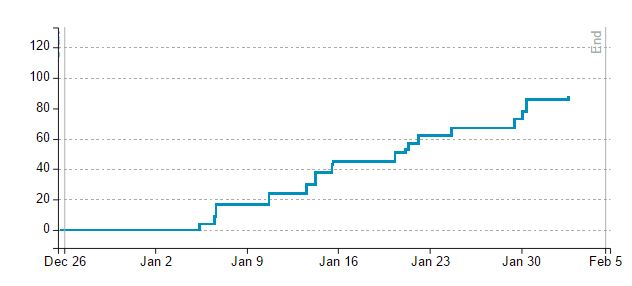
\includegraphics[width=1\linewidth]{gfx/Agilefant_Beta.jpg}
	\caption{Workload Distribution for Beta Release (23.12.2016-02.02.2017)}
	\label{fig:agilefant_beta}
\end{figure}

Figure~\ref{fig:agilefant_beta} shows the distribution of the workload over the time for the beta release. We see that there was no activity during the last week of December and first week of January (other than planned). The weeks after that are roughly evenly distributed. 
In total we already spent 194 hours (20h initiation + 86h alpha + 88h beta) on this project, such that we have 66 hours left. We are planning to use this time to implement \ac{SSTV}, finalize the documentation and to prepare the final presentation. 



\section{Final Release: 09.03.2017}
\label{sec:progress:final}




In this final release, we completed the documentation and prepared the final presentation. Other than initially planned, we decided after the beta release to implement \ac{SSTV} instead of improving \ac{BPSK} and implementing \ac{QAM}. Therefore, the expected workloads for those features became irrelevant. We estimated that we would be able to implement the SSTV feature in 50 hours.
\begin{table}[!htbp]
	\centering
	\caption{Expected and Actual Workload for Features in final Release}
	\label{tab:final:features}
	\begin{tabular}{ l | c | c }
		& expected  & actual \\ \hline
		SSTV & 50h & 58h+ \\  \hline
		Documentation & 25h & 21h \\ \hline \hline
		Presentation & 15h & 15h \\ \hline \hline 
		Total & 90h & 94h  
	\end{tabular}
\end{table}

Table~\ref{tab:final:features} shows the actual workload for this release. We see that we spent 58 hours on the SSTV feature and there are still parts that are currently not working properly. The documentation and presentation have been completed in the expected time, but other than initially planned we spent a good amount on the documentation in the previous releases. Therefore, the total documentation time is higher than expected. 

\begin{figure}[!htbp]
	\centering
	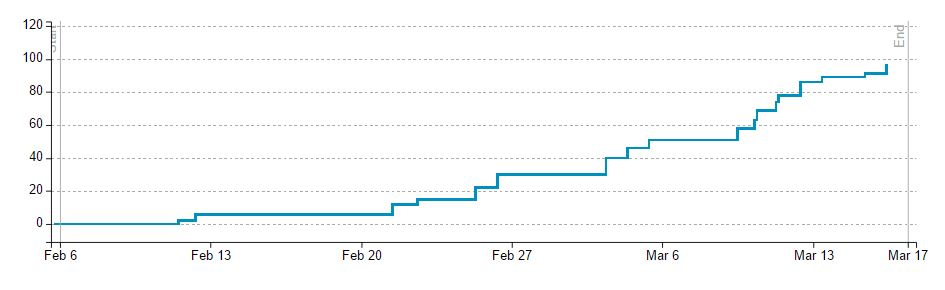
\includegraphics[width=1\linewidth]{gfx/Agilefant_Final.jpg}
	\caption{Workload Distribution for Final Release (03.02.2017-17.03.2017)}
	\label{fig:agilefant_final}
\end{figure}

Figure~\ref{fig:agilefant_final} shows the distribution of the workload over the time frame. The majority of the work was done in the last 3 weeks, due to other exams and vacation. 

